\subsection{Proof of Correctness}  
\label{sec:proof-th1}

We now provide the proof to support the correctness of the response time analysis presented in
Theorem~\ref{theorem:general-framework}, whatever the binary values
used in vector $\vec{x}$.  %The proof strategy is to
%show that the worst-case response time of task $\tau_k$ can be safely
%upper-bounded by any assignment of $\vec{x}$ of the $k-1$
%higher-priority tasks when adopting
%Eq.~(\ref{eq:TDA-suspension-tighter0}) as the response time analysis.
Throughout the proof, we consider any arbitrary assignment
$\vec{x}$, in which $x_i$ is either $0$ or $1$. For the sake of clarity, we classify the $k-1$
higher-priority tasks into two sets: ${\bf T}_0$ and ${\bf T}_1$. A
task $\tau_i$ is in ${\bf T}_0$ if $x_i$ is $0$; otherwise, it is in
${\bf T}_1$.




Our analysis is also based on very simple properties and lemmas enunciated as follows:

\begin{Property}
\label{prop:lower-priority}
In a preemptive fixed-priority schedule, the lower-priority jobs do not impact the schedule of the higher-priority jobs.
\end{Property}

%\begin{lemma}
%\label{lemma:remove-lower-priority}
%In a preemptive fixed-priority schedule, removing a lower-priority job arrived at time $t$ does not affect the schedule of the higher-priority jobs after time $t$.
%\end{lemma}
%\begin{proof}
%This is a direct consequence of Property~\ref{prop:lower-priority}.
%\end{proof}

\begin{Lemma}
\label{lemma:remove-same-task}
In a preemptive fixed-priority schedule, if the worst-case response
time of task $\tau_i$ is no more than its period $T_i$, removing a job of task $\tau_i$ does not affect the schedule of any other jobs of task $\tau_i$.
\end{Lemma}
\begin{proof}
Due to space limitation, the proof is\citetechreport{}.
\end{proof}


With the above properties, we can present the detailed proof of
Theorem~\ref{theorem:general-framework}. Since the proof is pretty long, we 
will also provide examples to demonstrate the key steps in the proof and lemmas to explain the intermediate conclusion in the proof.

\begin{appProof}{Theorem~\ref{theorem:general-framework}}
Consider the modified task set $\tau'$ composed of $\left\{\tau_1, \tau_2, \ldots, \tau_{k-1}, \tau_k', \tau_{k+1}, \ldots \right\}$ where $\tau_k' = (C_k + S_k, 0, D_k, T_k)$. Let $\Psi$ be a fixed-priority preemptive schedule of $\tau'$ such that $R_k' \leq T_k$.  
Suppose that a job $J_{k}$ of task $\tau_k'$ arrives at time $r_k$ and finishes at time $f_k$. 
By the assumption, we have $f_k \leq r_k+R_k' \leq r_k+T_k$.
We prove that Eq.~\eqref{eq:TDA-suspension-tighter0} gives us a safe upper bound on $f_k-r_k$ for any job $J_k$ in $\Psi$.


The proof is built upon the three following steps:
\begin{enumerate}
\item We discard all the jobs that arrive before $r_k$ and do not contribute to the response time of $J_k$ in the schedule $\Psi$. We follow an inductive strategy by iteratively inspecting the schedule of the higher priority tasks in $\Psi$, starting with $\tau_{k-1}$ until the highest priority task $\tau_1$. At each iteration, a time instant $t_j$ is identified such that $t_j \leq t_{j+1}$ ($1 \leq j < k$). Then, all the jobs of task $\tau_j$ released before $t_j$ are removed from the schedule and, if needed, replaced by an artificial job mimicking the interference caused by the residual workload of task $\tau_j$ at time $t_j$. %on the response time of job $J_k$. 
\item The final reduced schedule is analyzed so as to characterize the
  worst-case response time of $\tau_k'$ in $\Psi$. %by using workload functions.
\item We then prove that the response time analysis in Eq.~(\ref{eq:TDA-suspension-tighter0}) is indeed an upper bound on the worst-case response time $R_k'$ of $\tau_k'$.
\end{enumerate}

%!!!!!*************!!!!!!!!\\
%Since the proof involves several transformation steps. To illustrate some important steps in
%the proof, we also provide one concrete example. Consider a task
%system with 
%\begin{itemize}
%\item $T_1 = 6, C_1 = 1, S_1 = 1, x_1=1$,
%\item $T_2 = 10, C_2 = 1, S_2 = 6, x_2=0$,
%\item $T_3 = 18, C_3 = 4, S_3 = 1, x_3=1$,
%\item $T_4 = 20, C_4 = 5, S_4 = 0$.
%\end{itemize}
  
%!!!!!*************!!!!!!!!


\begin{figure*}[t]
  \centering
  \subfloat[$\Psi$, $\Psi^4$ and $\Psi^3$]{
    \scalebox{0.65}{
      
		\def\ux{0.5cm}\def\uy{0.5cm} 
		\begin{tikzpicture}[x=\ux,y=\uy, font=\sffamily,thick]  
		\tikzset{
			task/.style={fill=#1,  rectangle, text height=.3cm},
			task1a/.style={task=green!30},
			task1b/.style={task=green},
			task2a/.style={task=orange!30},
			task2b/.style={task=orange, minimum width=1mm},
			task3a/.style={task=pink, minimum width=1mm},
			task3b/.style={task=pink!80, minimum width=1mm},
			task4a/.style={task=cyan, minimum width=1mm},
			task4b/.style={task=cyan!50},
			task5/.style={task=blue},
			task6/.style={task=purple},
			task7/.style={minimum height=0.3cm,draw},
			task8/.style={minimum height=\ux,draw,thick},
			task9/.style={task=gray,minimum height=0.7cm,draw},
		}
		\tikzstyle{jobs}=[ fill=black!50];

		\begin{scope}[shift={(0,0)}]
		
		\draw[<-](4.1,1.1) -- (4.1,0);
		\draw[<->](10.1,1.1) -- (10.1,0);
		\draw[<->](16.1,1.1) -- (16.1,0);
		\draw[<->](22.1,1.1) -- (22.1,0);
		
		
		\draw[->] (0,0) node[anchor=east] {$\tau_1$}-- coordinate (xaxis) (25,0);

		
		\node[task7, minimum width=\ux,
		anchor=south west]at (5.1, 0){};
		\node[task7, minimum width=\ux,
		anchor=south west]at (10.1, 0){};
		\node[task7, minimum width=\ux,
		anchor=south west]at (16.1, 0){};
		\node[task7, minimum width=\ux,
		anchor=south west]at (22.1, 0){};
		\draw[(-), thin] (4.1, 0.3) -- (5.1, 0.3);

		\end{scope}
		
		
		\begin{scope}[shift={(0,-1.8)}]
		%%timeline
		
		
		\draw[<-](0,1.1) -- (0,0);
		\draw[<-](10,1.1) -- (10,0);
		\draw[<-](20,1.1) -- (20,0);
		
		
		\draw (6.1,0) -- (6.1, 0.3cm) -- (6.2, 0.3cm) --
                (6.2, 0);
		anchor=south west]  at ( 6, 0){};
		\node[task7, minimum width=0.9*\ux,
		anchor=south west] at (7, 0){};
		\draw (10,0) -- (10, 0.3cm) -- (10.1, 0.3cm) --
                (10.1, 0);
		\node[task7, minimum width=0.9*\ux,
		anchor=south west] at (11.1, 0){};
		\node[task7, minimum width=\ux,
		anchor=south west] at (21, 0){};

		\draw[->] (0,0)node[anchor=east] {$\tau_2$} -- coordinate (xaxis) (25,0);
		\draw[(-), thin] (0, 0.3) -- (5.1, 0.3);
		\draw[(-), thin] (6.2, 0.3) -- (7, 0.3);
		\draw[(-), thin] (20, 0.3) -- (21, 0.3);
		
		
		\end{scope}

		\begin{scope}[shift={(0,-3.6)}]
		%%timeline
		
		\draw[<-](6,1.1) -- (6,0);
		\draw[<-](24,1.1) -- (24,0);
		

		\draw[->] (0,0)node[anchor=east] {$\tau_3$} -- coordinate (xaxis) (25,0);
		
		\node[task7, minimum width=2.1*\ux,
		anchor=south west]  at ( 7.9, 0){};
		\node[task7, minimum width=1.9*\ux,
		anchor=south west]  at ( 12, 0){};
		
		\draw[(-), thin] (6, 0.3) -- (7, 0.3);
		
		\end{scope}

		\begin{scope}[shift={(0,-5.4)}]
		
		
		
		\draw[->] (0,0) node[anchor=east] {$\tau_4$}-- coordinate (xaxis) (25,0);
		\draw[<-](7,1.1) -- (7,0)node[anchor=north] {$$};
                \node[task7, minimum width=2.2*\ux,anchor=south west]at (13.9, 0){};
                \node[task7, minimum width=2.8*\ux,anchor=south west]at (17.1, 0){};
		
		\foreach \x in {0,...,24}{
			\draw[-](\x,0.1) -- (\x,-0.1)
			node[below] {\small $\x$};
			\draw[-,very thin, dotted](\x,6.5) -- (\x,-0.1);
		}


                \draw (19.9, -1.5) node {\small $f_4$};
                \draw (7, -1.5) node {\small $t_4$};
                \draw (6, -1.5) node {\small $t_3$};
                \draw (6, -2.1) node {\small .};
%                \draw (6, -2) node {\small $t_2$};
%                \draw (4.3, -1.5) node {\small $t_1$};
		\end{scope}
		
		\end{tikzpicture}  
}}
  \subfloat[$\Psi^2$ and $\Psi^1$]{
    \scalebox{0.65}{
      
		\def\ux{0.5cm}\def\uy{0.5cm} 
		\begin{tikzpicture}[x=\ux,y=\uy, font=\sffamily,thick]  
		\tikzset{
			task/.style={fill=#1,  rectangle, text height=.3cm},
			task1a/.style={task=green!30},
			task1b/.style={task=green},
			task2a/.style={task=orange!30},
			task2b/.style={task=orange, minimum width=1mm},
			task3a/.style={task=pink, minimum width=1mm},
			task3b/.style={task=pink!80, minimum width=1mm},
			task4a/.style={task=cyan, minimum width=1mm},
			task4b/.style={task=cyan!50},
			task5/.style={task=blue},
			task6/.style={task=purple},
			task7/.style={minimum height=0.3cm,draw},
			task8/.style={minimum height=\ux,draw,thick},
			task9/.style={task=gray,minimum height=0.7cm,draw},
		}
		\tikzstyle{jobs}=[ fill=black!50];

		\begin{scope}[shift={(0,0)}]
		
		\draw[<-](4.1,1.1) -- (4.1,0);
		\draw[<->](10.1,1.1) -- (10.1,0);
		\draw[<->](16.1,1.1) -- (16.1,0);
		\draw[<->](22.1,1.1) -- (22.1,0);
		
		
		\draw[->] (0,0) node[anchor=east] {$\tau_1$}-- coordinate (xaxis) (25,0);

		
		\node[task7, minimum width=\ux,
		anchor=south west]at (5.1, 0){};
		\node[task7, minimum width=\ux,
		anchor=south west]at (10.1, 0){};
		\node[task7, minimum width=\ux,
		anchor=south west]at (16.1, 0){};
		\node[task7, minimum width=\ux,
		anchor=south west]at (22.1, 0){};
		\draw[(-), thin] (4.1, 0.3) -- (5.1, 0.3);

		\end{scope}
		
		
		\begin{scope}[shift={(0,-1.8)}]
		%%timeline
		
		
		\draw[<-](6,1.1)
                node[anchor=west,xshift=-3.1cm,yshift=0.1cm]{\footnotesize\textcolor{blue}{release
                    an artifical job of $\tau_2$ at time $6$}} -- (6,0);
		\draw[<-](10,1.1) -- (10,0);
		\draw[<-](20,1.1) -- (20,0);
		
		
		\draw (6.1,0) -- (6.1, 0.3cm) -- (6.2, 0.3cm) --
                (6.2, 0);
		anchor=south west]  at ( 6, 0){};
		\node[task7, minimum width=0.9*\ux,
		anchor=south west] at (7, 0){};
		\draw (10,0) -- (10, 0.3cm) -- (10.1, 0.3cm) --
                (10.1, 0);
		\node[task7, minimum width=0.9*\ux,
		anchor=south west] at (11.1, 0){};
		\node[task7, minimum width=\ux,
		anchor=south west] at (21, 0){};

		\draw[->] (0,0)node[anchor=east] {$\tau_2$} -- coordinate (xaxis) (25,0);
%		\draw[(-), thin] (0, 0.3) -- (5.1, 0.3);
		\draw[(-), thin] (6.2, 0.3) -- (7, 0.3);
		\draw[(-), thin] (20, 0.3) -- (21, 0.3);
		
		
		\end{scope}

		\begin{scope}[shift={(0,-3.6)}]
		%%timeline
		
		\draw[<-](6,1.1) -- (6,0);
		\draw[<-](24,1.1) -- (24,0);
		

		\draw[->] (0,0)node[anchor=east] {$\tau_3$} -- coordinate (xaxis) (25,0);
		
		\node[task7, minimum width=2.1*\ux,
		anchor=south west]  at ( 7.9, 0){};
		\node[task7, minimum width=1.9*\ux,
		anchor=south west]  at ( 12, 0){};
		
		\draw[(-), thin] (6, 0.3) -- (7, 0.3);
		
		\end{scope}

		\begin{scope}[shift={(0,-5.4)}]
		
		
		
		\draw[->] (0,0) node[anchor=east] {$\tau_4$}-- coordinate (xaxis) (25,0);
		\draw[<-](7,1.1) -- (7,0)node[anchor=north] {$$};
                \node[task7, minimum width=2.2*\ux,anchor=south west]at (13.9, 0){};
                \node[task7, minimum width=2.8*\ux,anchor=south west]at (17.1, 0){};
		
		\foreach \x in {0,...,24}{
			\draw[-](\x,0.1) -- (\x,-0.1)
			node[below] {\small $\x$};
			\draw[-,very thin, dotted](\x,6.5) -- (\x,-0.1);
		}


                \draw (19.9, -1.5) node {\small $f_4$};
                \draw (7, -1.5) node {\small $t_4$};
                \draw (6, -1.5) node {\small $t_3$};
                \draw (6, -2) node {\small $t_2$};
                \draw (4.3, -1.5) node {\small $t_1$};
		\end{scope}
		
		\end{tikzpicture}  
}}
\caption{An illustrative example of Step 1 in the proof of Theorem~\ref{theorem:general-framework} when $\epsilon = 0.1$.}
\label{fig:example}  
\end{figure*}


\noindent{\bf Step 1 in our proof: Reducing the schedule $\Psi$} 

\emph{Our purpose in this step is to discard all the jobs that arrive before $r_k$ and have no impact on the response time of $J_k$ in the schedule
  $\Psi$. } During this step, we iteratively build an artificial schedule $\Psi^j$ from $\Psi^{j+1}$ (with $1 \leq j < k$) so that the response time of $\tau_{k}'$ remains identical. At each iteration, we define $t_j$ for task $\tau_j$ in the schedule $\Psi^{j+1}$ (with $j=k-1, k-2, \ldots, 1$) and build $\Psi^j$ by removing all the jobs released by $\tau_j$ before $t_j$. \emph{Therefore, the correctness of this step is to show that the response time of $J_k$ in the original schedule $\Psi$ remains the same as the response time of $J_k$ in  the reduced schedule $\Psi^1$.}


\noindent\textit{Basic step (definition of $\Psi^k$ and $t_k$):} 

Recall that the job $J_{k}$ of task $\tau_k'$ arrives at time $r_k$ and finishes at time $f_k$ in schedule $\Psi$. We know by Property~\ref{prop:lower-priority} that the lower priority tasks $\tau_{k+1}, \tau_{k+2}, \ldots, \tau_n$ do not impact the response time of $J_{k}$. Moreover, since we assume that the worst-case response time of task $\tau_k'$ is no more than $T_k$, Lemma~\ref{lemma:remove-same-task} proves that removing all the jobs of task $\tau_k'$ but $J_{k}$ has no impact on the schedule of $J_{k}$. Therefore, let $\Psi^k$ be a schedule identical to $\Psi$ but removing all the jobs released by the lower priority tasks $\tau_{k+1}, \ldots, \tau_n$ as well as all the jobs released by $\tau_k'$ at the exception of $J_{k}$. The response time of $J_{k}$ in $\Psi^{k}$ is identical to the response time of $J_{k}$ in $\Psi$.

We define $t_k$ as the release time of $J_k$ (i.e., $t_k = r_k$).


\noindent\textit{Induction step (definition of $\Psi^j$ and $t_j$ with $1 \leq j < k$):}

Let $r_j$ be the arrival time of the last job released by $\tau_j$ before $t_{j+1}$ in $\Psi^{j+1}$ and let $J_{j}$ denote that job. By definition, $r_j < t_{j+1}$. %There are a two possible cases:
%\begin{itemize}
%\item $J_{j}$ completed its execution no later than $t_{j+1}$. Then, we simply set $t_j$ to $t_{j+1}$ and generate $\Psi^j$ by removing all the jobs of task $\tau_j$ arrived before $t_{j+1}$ in the schedule $\Psi^{j+1}$. By Lemma~\ref{lemma:remove-same-task} and Property \ref{prop:lower-priority}, removing all the jobs of task $\tau_j$ arrived before $t_{j+1}$ has no impact on the schedule of the higher-priority jobs (jobs released by $\tau_1, \ldots, \tau_{j-1}$) and the jobs of $\tau_j$ released after $t_{j+1}$. Moreover, because no task with a priority lower than $\tau_j$ executes jobs before $t_{j+1}$ in $\Psi^{j+1}$, removing the jobs released by $\tau_j$ before $t_{j+1}$ does not impact the schedule of the jobs of $\tau_{j+1}, \ldots, \tau_{k}$. The response time of $J_{k}$ in $\Psi^j$ thus remains unchanged in comparison to its response time in $\Psi^{j+1}$. 
%\item $J_{j}$ did not complete its execution before $t_{j+1}$.
If $r_j$ does not exist, i.e., all the jobs of task $\tau_j$ are released at  or after $t_{j+1}$, then, we can safely set $\Psi^j$ as $\Psi^{j+1}$ and $t_j$ as $t_{j+1}$. This does not change the response time of $J_k$ since the schedules $\Psi^j$ and $\Psi^{j+1}$ are the same. For such a case, the induction step for task $\tau_j$ finishes. 

For the rest of the induction step, we focus on the other case, i.e., $r_j$ exists.
\emph{By the assumption that $R_j \leq D_j \leq T_j$ for $j=1,2,\ldots,k-1$}, removing all the jobs of task $\tau_j$ arrived before $r_j$ has no impact on the schedule of any other job released by $\tau_j$ (Lemma~\ref{lemma:remove-same-task}) or any higher priority job released by $\tau_1, \ldots, \tau_{j-1}$ (Property \ref{prop:lower-priority}). Moreover, because by the construction of $\Psi^{j+1}$, no task with a priority lower than $\tau_j$ executes jobs before $t_{j+1}$ in $\Psi^{j+1}$, removing the jobs released by $\tau_j$ before $t_{j+1}$ does not impact the schedule of the jobs of $\tau_{j+1}, \ldots, \tau_{k}$. \emph{Therefore, we can safely remove all the jobs of task $\tau_j$ arrived before $r_j$ without impacting the response time of $J_{k}$.}

But, should we include or exclude $J_j$ for the construction of
$\Psi^j$?  We use three rules to define the construction of the
schedule $\Psi^j$ and $t_j$ for including or excluding $J_j$.
\begin{compactitem}
\item {\bf Rule 1 assigns $t_j$ to $r_j$ by including $J_j$:} This rule is applied to
  include the complete job of task $\tau_j$ released at time $r_j$
  in the schedule $\Psi^j$. 
\item {\bf Rule 2 assigns $t_j$ to $t_{j+1}$ by excluding $J_j$:} This rule is applied to
  completely exclude $J_j$ in the schedule $\Psi^j$. 
\item {\bf Rule 3 assigns $t_j$ to $t_{j+1}$ by partially excluding
    $J_j$:} This rule is applied to partially exclude $J_j$ in the
  schedule $\Psi^j$.  If we apply this rule, we will remove $J_j$ and
  create an artificial job to represent the residual workload of $J_j$
  (to be explained and defined later), executed at or after $t_{j+1}$.
\end{compactitem}

We apply the above three rules, depending on different cases, as follows:
\begin{enumerate}[(a)]
\item $\tau_j \in {\bf T}_1$: In this case, we analyze two different subcases:
\begin{itemize}
\item $J_{j}$ does not complete its execution by $t_{j+1}$ in schedule $\Psi^{j+1}$. For such a case, {\bf Rule 1} is applied. Therefore, $t_{j}$ is set to $r_j$ and $\Psi^j$ is built from $\Psi^{j+1}$ by removing all the jobs released by $\tau_j$ before $r_j$.  \emph{Clearly, this has no impact on the execution of any job executed after $t_j$ and thus on the response time of $J_k$.}
\item $J_{j}$ completes its execution before or at $t_{j+1}$ in schedule $\Psi^{j+1}$. For such a case, {\bf Rule 2} is applied.  By Lemma~\ref{lemma:remove-same-task} and Property \ref{prop:lower-priority}, removing all the jobs of task $\tau_j$ arrived before $t_{j+1}$ has no impact on the schedule of the higher-priority jobs (jobs released by $\tau_1, \ldots, \tau_{j-1}$) and the jobs of $\tau_j$ released after or at $t_{j+1}$. 
Moreover, because no task with lower priority than $\tau_j$ executes jobs before $t_{j+1}$ in $\Psi^{j+1}$, removing the jobs released by $\tau_j$ before $t_{j+1}$ does not impact the schedule of the jobs of $\tau_{j+1}, \ldots, \tau_{k}$. Therefore, $t_j$ is set to $t_{j+1}$ and $\Psi^j$ is generated by removing all the jobs of task $\tau_j$ arrived before $t_{j+1}$. \emph{The response time of $J_{k}$ in $\Psi^j$ thus remains unchanged in comparison to its response time in $\Psi^{j+1}$.}
\end{itemize}
\item If $\tau_j \in {\bf T}_0$: For such a case, we set $t_{j}$ to $t_{j+1}$ by applying {\bf Rule 3}. Let $c_j^*$ be the remaining execution time for the job of task $\tau_j$ at time $t_j$. By definition, $c_j^* \geq 0$, and we also know that $c_j^*$ is at most $C_j$. Since by the construction of $\Psi^j$, all the jobs of $\tau_j$ released before $t_j$ are removed, the job of task $\tau_j$ arrived at time $r_j$ ($< t_j$) is replaced by a new job released at time $t_j$ with execution time $c_j^*$ and the same priority than $\tau_j$. \emph{Clearly, this has no impact on the execution of any job executed after $t_j$ and thus on the response time of $J_k$.} The remaining execution time $c_j^*$ of $\tau_j$ at time $t_j$ is called the \emph{residual workload} of task $\tau_j$ in the rest of the proof.
\end{enumerate}
%\end{itemize}

 
\noindent\textit{Conclusion of Step 1}:

This iterative process is repeated until producing $\Psi^1$. The procedures are well-defined and it is therefore guaranteed that $\Psi^1$ can be constructed, in which the procedure can be found in Appendix\citetechreport{}.  Note that after each iteration, the number of jobs considered in the resulting schedule has been reduced, yet without affecting the response time of $J_k$. We conclude the first step by the following lemma.

 \begin{Lemma}
\label{lem:step-1-conclusion}
 The response time of job $J_k$ in $\Psi^1$ is the same as the response time of $J_k$ in $\Psi$.
\end{Lemma}
\begin{proof}
  This has been explicitly proven by the above induction hypothesis.
\end{proof}


\begin{example}
\label{ex:proof_step1}
Consider 4 tasks $\tau_1 =(1,1,6,6)$, $\tau_2 =(1,6,10,10)$, $\tau_3 =(4,1,18,18)$ and $\tau_4 =(5,0,20,20)$.
We assume  $x_1=1$, $x_2=0$, $x_3=1$ in this example.
Figure~\ref{fig:example}(a) depicts a possible schedule $\Psi^4$ of those tasks. We assume that the first job of task $\tau_1$ arrives
at time $4+\epsilon$ with $0 < \epsilon < 0.5$. The first job
of task $\tau_2$ suspends itself from time $0$ to time $5+\epsilon$,
and is blocked by task $\tau_1$ from time $5+\epsilon$ to time
$6+\epsilon$. After executing $\epsilon$ amount
of time, the first job of task $\tau_2$ suspends itself again from
time $6+2\epsilon$ to $7$. The schedule in Figure~\ref{fig:example}(a) is drawn for $\epsilon=0.1$.
   
In the schedule illustrated in Figure~\ref{fig:example}(a), $f_4$ is
$20-\epsilon$, i.e., $f_4=19.9$ when $\epsilon=0.1$.  We define $t_4$
as $7$. Then, we set $t_3$ to $6$ by applying {\bf Rule 1}. The
schedule $\Psi^3$ is identical to the original schedule $\Psi^4$.

When considering task $\tau_2$, we know that $J_2$ is the job of task
$\tau_2$ arrived at time $r_2=0 < t_3$. Since task $\tau_2$ belongs to ${\bf
  T}_0$, by applying {\bf Rule 3}, we set $t_2$ to $t_3=6$ and the
residual workload $c_2^*$ is $1$. Then, we remove job $J_2$ from the
schedule and create an artificial job with execution time $c_2^*$ that
is released at time $t_2$ and assign the artificial job the same priority level as task
$\tau_2$. Note that this artificial job can still suspend itself. Therefore, the schedule $\Psi^2$, as drawn in 
Figure~\ref{fig:example}(b), is slightly different from $\Psi^3$, shown in Figure~\ref{fig:example}(a).

Then, $t_1$ is set to $4+\epsilon$ by applying {\bf Rule 1} since
$J_1$ (arrived at time $r_1=4+\epsilon$) has not completed yet at time
$t_2=6$.  The schedule $\Psi^1$ is identical to the schedule
$\Psi^2$.
% We have to further consider one job of task $\tau_2$ arrived
% before time $t_1$ with execution time $C_2$. 
\myendproof
\end{example}

\noindent{\bf Step 2 in our proof: Analyzing the reduced schedule $\Psi^1$}

We now analyze the properties of the final schedule $\Psi^1$ in which
all the unnecessary jobs have been removed. The main purpose of this
step is to prove the correctness of the conditions listed in
Lemma~\ref{lemma:conclusion-step2} for the schedule $\Psi^1$. 

By Lemma~\ref{lem:step-1-conclusion}, the response time of job $J_k$ is the same in both schedules $\Psi$ and $\Psi^1$.
The proof is based on the fact that for any interval $[t_1, t)$ with $t \leq f_k$, there is 
\begin{equation}
\label{eq:exec_plus_idle}
\operatorname{idle}(t_1, t) + \operatorname{exec}(t_1, t)  = (t - t_1)
\end{equation}
where $\operatorname{exec}(t_1, t)$ is the amount of time during which the processor executes tasks within $[t_1, t)$, and $\operatorname{idle}(t_1, t)$ is the amount of time during which the processor remains idle within the interval $[t_1, t)$.




%If $t_i < t_{i+1}$, the processor may idle in the time interval $[t_i,
%t_{i+1})$ in $\Psi^1$. 
%Let $\sigma_i$ be the total idle time in $\Psi^1$ within the time interval $[t_i, t_{i+1})$. 

We start our analysis with $\operatorname{idle}(t_1, t)$ when $t_1 < t \leq f_k$.
Let $\sigma_j$ be the amount of time during which the processor remains idle within $[t_j, t_{j+1})$ in $\Psi^1$. If $t_j$ is equal to $t_{j+1}$, by definition, $\sigma_j$ is $0$.
We have the following lemma:
\begin{Lemma}
\label{lem:max_idle}
$\sum_{j=1}^{i-1} \sigma_j  = \sum_{j=1}^{i-1} x_j \sigma_j\leq \sum_{j=1}^{i-1} x_j S_j$. %$\sigma_j \leq S_j$.
\end{Lemma}
\begin{proof}
  For $j=1,2,\ldots,k-1$, 
  since $\sigma_j$ is $0$ if $t_j$ is equal to $t_{j+1}$, we only have
  to consider the case when {\bf Rule 1} is applied for setting $t_j$
  in Step 1, i.e., $x_j$ must be $1$.  When {\bf Rule 1} is applied for task $\tau_j$ in Step 1, $t_j$ is set to $r_j$ and
  the job $J_j$ has not completed its execution yet at time $t_{j+1}$. Therefore, the
  amount of time during which the processor may remain idle within
  $[t_j, t_{j+1})$ is at most $S_j$ time units, i.e., $\sigma_j \leq S_j$.   It results that
  $\sum_{j=1}^{i-1} \sigma_j = \sum_{j=1}^{i-1} x_j \sigma_j \leq
  \sum_{j=1}^{i-1} x_j S_j$.
\end{proof}

From Lemma~\ref{lem:max_idle}, it holds that, for $i=2,3,\ldots,k$, $\forall t | t_{i-1} < t \leq t_i$, 
\begin{align}
\label{eq:sumof-sigma}
%\operatorname{idle}(t_1, t) \leq \sum_{i: t_i < t} \sigma_i
\operatorname{idle}(t_1, t) = \sum_{j=1}^{i-1} x_j \sigma_j \leq
  \sum_{j=1}^{i-1} x_j S_j
\end{align}

As shown in the schedule in Example~\ref{ex:proof_step1}, the total idle time from $4+\epsilon$ to
$20-\epsilon$, i.e., from $4+\epsilon$ to $5+\epsilon$ and from
$6+2\epsilon$ to $7$, is $2-2\epsilon$, which is upper-bounded by $2 =
S_1+S_3$. 


% by JJ 23,04,2016 -> this following step seems to be not useful. 
%
% Moreover, by the definition of $t_k$ and $f_k$, the schedule $\Psi^1$
% does not have any idle time between $t_k$ and $f_k$. Therefore, 
% it holds that $\forall t | t_k < t \leq f_k$, 
% \begin{align}
% \label{eq:sumof-sigma-2}
% %\operatorname{idle}(t_1, t) \leq \sum_{i: t_i < t} \sigma_i
% \operatorname{idle}(t_1, t) \leq \sum_{j=1}^{k-1} x_j S_j.
% \end{align}
% The above two cases can be found in the example in Figure~\ref{fig:example}.

%From Lemma~\ref{lem:max_idle}. %If $t_i$ is equal to $t_{i+1}$, then $\sigma_i$ is set to $0$. 

We now consider $\operatorname{exec}(t_1, t)$ when $t_1 < t \leq f_k$.
Because there is no job released by lower priority tasks than
$\tau_k'$ in $\Psi^1$, we only focus on the execution patterns of the
tasks $(\tau_1, \tau_2, \ldots, \tau_{k-1}, \tau_k')$. Let
$\operatorname{exec}_j(t_1, t)$ be the workload, defined as \emph{the
 (accumulative) amount of time that task $\tau_j$ is executed in the schedule
  $\Psi^1$ in the time interval $(t_1, t]$}. By the definition of the
schedule $\Psi^1$, we know that $\operatorname{exec}_j(t_1, t_j)$ must
be $0$. Therefore, $\operatorname{exec}_j(t_1, t)$ is equal to
$\operatorname{exec}_j(t_j, t)$ if $t > t_j$.

\begin{Lemma}
  \label{lemma:exec-tau-k}
  $\forall t | t_k \leq t < f_k$, the (accumulative) amount of time that
  task $\tau_k'$ is executed from $t_k$ to $t$ is $\operatorname{exec}_k(t_k, t) <
  C_k$.
\end{Lemma}
\begin{proof}
  Since the finishing time of job $J_k$ is at time $f_k$ in schedule $\Psi^1$, the
  condition holds by definition.
\end{proof}

According to Step 1, we should consider three rules when analyzing $\operatorname{exec}_j(t_j, t)$ for $j=1,2,\ldots,k-1$:
\begin{itemize}
\item Task $\tau_j$ applies {\bf Rule 1}. This is the case when
  $\tau_j \in {\bf T}_1$ and the job $J_j$ has not finished yet at
  time $t_{j+1}$. In this case, there is no job of task $\tau_j$
  arrived before $t_j$ in $\Psi^1$.  Therefore, for any $\Delta \geq
  0$, the workload $\operatorname{exec}_j(t_j, t_j+\Delta)$, executed by $\tau_j$ on the
  processor from $t_j$ to $t_j+\Delta$ is upper bounded by a function $\operatorname{exec}_j(t_j, t_j+\Delta)  \leq W_j^1(\Delta)$, defined as follows:
{\footnotesize \begin{equation}
  \label{eq:execution-case1}
  W_j^1(\Delta) \stackrel{\mbox{def}}{=} \floor{\frac{\Delta}{T_j}}C_j + \min\left\{\Delta-\floor{\frac{\Delta}{T_j}}T_j, C_j\right\}.
\end{equation}}The above workload function in Eq.~\eqref{eq:execution-case1} has been widely used in the literature if task $\tau_j$ is an ordinary sporadic task without self-suspension, e.g., in \cite{bertogna2006new}. However, since we are only interested to get an upper bound  of $\operatorname{exec}_j(t_j, t_j+\Delta)$, it is obvious that self-suspension does not play any specific rule here.

\item Task $\tau_j$ applies {\bf Rule 2}. This is the case when
  $\tau_j \in {\bf T}_1$ and the job $J_j$ already finishes at time
  $t_{j+1}$. In this case, it is clear that $\operatorname{exec}_j(t_j, t_j+\Delta)  \leq W_j^1(\Delta)$ also holds.

\item Task $\tau_j$ applies {\bf Rule 3}. This is the case when
  $\tau_j \in {\bf T}_0$. There might be a job $J_j$ arrived before
  $t_j$ with the residual workload $0 \leq c_j^* \leq C_j$ at time
  $t_j$. For notational brevity, let $\rho_j$ be defined as $(T_j-R_j +
  c_j^*)$. We will show that $\operatorname{exec}_j(t_j, t_j+\Delta) \leq
  \widehat{W}_j^0(\Delta, c_j^*)$, defined as follows for two cases for $\Delta \geq 0$:
  If $c_j^*$ is $0$, then\footnote{The reader may think that this case
    is not necessary, but it is, since the formulation in
    Eq.~\eqref{eq:execution-case2-precise} does not cover this case.}
  \begin{equation}
  \label{eq:execution-case2-cj*=0}
 \widehat{W}_j^0(\Delta, 0)=    W_j^1(\Delta);
  \end{equation}
  otherwise if $c_j^* > 0$, then
  \begin{equation}
    \label{eq:execution-case2-precise}
    \widehat{W}_j^0(\Delta, c_j^*)=
    \begin{cases}
      \Delta & \mbox{ if } \Delta \leq  c_j^*\\
      c_j^* & \mbox{ if } c_j^* < \Delta \leq  \rho_j\\
      c_j^* + W_j^1(\Delta-\rho_j) & \mbox{ otherwise}.
    \end{cases}
  \end{equation}
  The case when $c_j^*$ is $0$ is easy to see, since this is identical to
  the case when {\bf Rule 2} is applied for task $\tau_j$. We now consider another case when $c_j^* > 0$.
  %Two subcases are considered:
  %\begin{itemize}
  %\item If the residual workload $c_j^*$
  %of task $\tau_j$ is $0$, the earliest next arrival time of task $\tau_j$
  %can be any time instant at or after $t_j$. 
%In this case, for any $\Delta \geq 0$, the workload $\widehat{W}_j^0(\Delta, c_j^*)$ executed by $\tau_j$ from $t_j$ to $t_j+\Delta$ is upper bounded by $W_j^1(\Delta)$. 
%\item If the residual workload $c_j^*$ of task $\tau_j$ is larger than $0$,
  Since by our assumption $R_j \leq D_j \leq T_j$, task $\tau_j$ respects all its deadlines and the
  worst-case response time, the finishing time of the job of $\tau_j$ (that has not finished yet at $t_j$) must be at least $t_j + c_j^*$; otherwise that job would violate its worst-case execution time (that has been confirmed earlier). Therefore, the earliest arrival time of task $\tau_j$
  arriving \emph{strictly after $t_j$} is at least $t_j + (T_j-R_j +
  c_j^*) = t_j+\rho_j$. Therefore, the workload function for such a case is like $W_j^1$ shifted by $\rho_j$ when $\Delta > \rho_j$.
\end{itemize}


\begin{Lemma}
\label{lemma:Wj01-exact}
$\forall \Delta \geq 0$ and given $c_j^*$ for a task $\tau_j \in {\bf T}_0$, we have 
\[
\begin{cases}
\operatorname{exec}_j(t_j, t_j+\Delta) \leq \widehat{W}_j^0(\Delta, c_j^*) &\mbox{ if } \tau_j \in {\bf T}_0\\  
\operatorname{exec}_j(t_j, t_j+\Delta) \leq W_j^1(\Delta) &\mbox{ if } \tau_j \in {\bf T}_1  
 \end{cases}
\]
\end{Lemma}
\begin{proof}
  Both cases have been discussed above.
\end{proof}
For a given $\Delta$, we can prove that $W_j^0(\Delta)\equals \widehat{W}_j^0(\Delta, C_j) \geq \widehat{W}_j^0(\Delta, c_j^*)$ as follows:
\begin{Lemma}
\label{lemma:Wj0-dominate}
$\forall \Delta \geq 0$ and $\forall C_j\geq c_j^* \geq 0$,
\[
W_j^0(\Delta)\equals \widehat{W}_j^0(\Delta, C_j)  \geq \widehat{W}_j^0(\Delta, c_j^*),
\]
where $\widehat{W}_j^0(\Delta, 0)$ is defined in \eqref{eq:execution-case2-cj*=0}  and
$\widehat{W}_j^0(\Delta, c_j^*)$ is defined in Eq.~(\ref{eq:execution-case2-precise}) if $c_j^* > 0$.
\end{Lemma}
\begin{proof}
 The proof is based on simple observations of the workload function. The proof is in Appendix\ifbool{techreport}{.}{\citetechreport{}.}
\end{proof}

% When $c_j^* > 0$, it is easy to see that
% Eq.~\eqref{eq:execution-case2-precise} is maximized when $c_j^*$ is
% maximum, that is, when $c_j^* = C_j$. When $c_j^* = 0$, due to the assumption of constrained-deadline task sets, it is also easy to see that 
% $\widehat{W}_j^0(\Delta, 0) = W_j^1(\Delta) \leq \widehat{W}_j^0(\Delta, C_j)$
% It results that for all $\Delta \geq 0$ and $0 \leq c_j^* \leq C_j$, we have $\widehat{W}_j^0(\Delta, C_j) \geq
% \widehat{W}_j^0(\Delta, c_j^*)$.


%For the sake of notational brevity,
%we introduce the notation $W_j^0(\Delta)$ defined as follows.
%\begin{equation}
%  \label{eq:execution-case2-upperbounded}
% W_j^0(\Delta) \equals \widehat{W}_j^0(\Delta, C_j) 
%\end{equation}

%For the sake of notational brevity, for the rest of this proof, we use the notation $W_j^0(\Delta)$ to denote $\widehat{W}_j^0(\Delta, C_j)$.
Now, we can safely reformulate the condition in Eq.~\eqref{eq:exec_plus_idle} to the conditions in the following lemma.
\begin{Lemma}
  \label{lemma:conclusion-step2}
For $i=2,3,\ldots,k-1$ that $\forall t \mid t_{i-1} \leq t < t_i$
\begin{equation}
\label{eq:exec_plus_idle-2}
\sum_{j=1}^{i-1} x_j\cdot (W_j^1(t-t_j) +\sigma_j) + (1-x_j)\cdot W_j^0(t-t_j) \geq t-t_1.
\end{equation}
 Moreover, $\forall t \mid t_k \leq t < f_k$,
\begin{equation}
\label{eq:exec_plus_idle-3}
C'_k +\sum_{j=1}^{k-1} x_j\cdot (W_j^1(t-t_j) +\sigma_j) + (1-x_j)\cdot W_j^0(t-t_j) > t-t_1.
\end{equation} 
\end{Lemma}
\begin{proof}
  By Lemmas~\ref{lemma:Wj01-exact}~and~\ref{lemma:Wj0-dominate} and the condition that $\vec{x}$
  is specified with only binary values in its elements, for
  $i=2,3,\ldots,k-1$ that $\forall t \mid t_{i-1} \leq t < t_i$, we
  have
{\small \begin{align}
\label{eq:exec_time}
\operatorname{exec}(t_1, t) \leq \sum_{j=1}^{i-1} x_j\cdot W_j^1(t-t_j)  + (1-x_j)\cdot W_j^0(t-t_j).
\end{align}} Injecting $\operatorname{idle}(t_1, t) = \sum_{j=1}^{i-1}
x_j \sigma_j $ from Eq.~(\ref{eq:sumof-sigma}) and the condition from
(\ref{eq:exec_time}) to Eq.~(\ref{eq:exec_plus_idle}), we can reach
the condition in Eq.~\eqref{eq:exec_plus_idle-2}.\footnote{\label{footnote-why-sigma}The readers
  may think of using the condition $\operatorname{idle}(t_1, t) \leq
  \sum_{j=1}^{i-1} x_j S_j$ in Eq.~\eqref{eq:sumof-sigma} to
  replace $\sigma_j$ with $S_j$. But, this will create a serious
  problem in Step 3 later, since we cannot always guarantee that
  $t_i^*\leq t_i$ for $i=1,2,\ldots,k$ in Step 3 if we do so in Step 2. Such a treatment should not be applied at this moment here.} 

Moreover, since $\tau_k'$ does not complete its execution
\emph{strictly} before $f_k$ and because, by definition, $\tau_k'$
does not self-suspend, we also know that $\operatorname{idle}(t_k,
f_k)$ is $0$. By Lemma~\ref{lemma:exec-tau-k} and the above
conditions, we reach the condition in Eq.~\eqref{eq:exec_plus_idle-3}.
\end{proof}




\begin{example}
Consider the same 4 tasks as in Example~\ref{ex:proof_step1}, for which a possible schedule was depicted in Figure~\ref{fig:example} when $\epsilon$ is very close to $0$. We have $x_1\sigma_1=1$, $x_2\sigma_2=0$ and $x_3\sigma_3=1-2\epsilon$. The corresponding functions
$W_1^1(t-t_1)$, $W_2^0(t-t_2)$, $W_3^1(t-t_3)$ are illustrated in
Figure~\ref{fig:example-step2} when $\epsilon$ is close to $0$. Here, we consider $R_2 = 10$. More precisely,

{\footnotesize \begin{compactitem}
  \item $W_1^1(t-t_1) = \floor{\frac{t-t_1}{6}}1 + \min\left\{t-t_1-\floor{\frac{t-t_1}{6}}6, 1\right\}$ if $t \geq t_1$.
  \item $W_2^0(t-t_2) = t-t_2$ if $t_2 \leq t \leq t_2 + 1$ and $W_2^0(t-t_2) = 1 + \floor{\frac{t-t_2-1}{10}} + \min\left\{t-t_2-1-\floor{\frac{t-t_2-1}{10}}10, 1\right\}$ if $t > t_2+1$.
  \item $W_3^1(t-t_3) = \floor{\frac{t-t_3}{18}}4 + \min\left\{t-t_3-\floor{\frac{t-t_3}{18}}18, 4\right\}$ if $t \geq t_3$.
\end{compactitem}
}As can be seen in the figure, the inequalities of Eqs.~\eqref{eq:exec_plus_idle-2} and~\eqref{eq:exec_plus_idle-3} clearly hold.\myendproof
\end{example}


Before moving to Step 3, the following lemma is useful for setting the workload upper bound.
\begin{Lemma}
  \label{lemma:W_0-and-W_1-upper}
For any $\Delta > 0$, we have
\begin{align}
  W_j^1(\Delta)  \leq &\ceiling{\frac{\Delta}{T_j}}C_j & \mbox{ if } \tau_j \in {\bf T}_1   \label{eq:W_1-upper}\\
  W_j^0(\Delta)  \leq &\ceiling{\frac{\Delta+R_j-C_j}{T_j}}C_j & \mbox{ if } \tau_j \in {\bf T}_0   \label{eq:W_0-upper}
\end{align}
\end{Lemma}
\begin{proof}
  The upper bound of $W_j^1(\Delta)$ is obvious. We focus on the upper bound of $W_j^0(\Delta)$. If $0 < \Delta \leq C_j$, we know that $W_j^0(\Delta) = \Delta \leq C_j \leq \ceiling{\frac{\Delta+R_j-C_j}{T_j}}C_j$. If $\Delta > C_j$, then 
{\small \begin{align*}
W_j^0(\Delta) &\leq_1 C_j + W_j^1(\Delta - (T_j-R_j+C_j))\nonumber\\
& \leq C_j+\ceiling{\frac{\Delta-T_j +(R_j-C_j)}{T_j}}C_j  = \ceiling{\frac{\Delta+R_j-C_j}{T_j}}C_j 
\end{align*}} where $\leq_1$ is achieved by Lemma~\ref{lemma:Wj0-dominate} and setting
$c_j^*$ to $C_j$ in Eq.~\eqref{eq:execution-case2-precise}.
\end{proof}

\noindent{\bf Step 3: Creating a Safe Response-Time Upper Bound}


\begin{figure}[t]
  \centering

		\def\ux{0.32cm}\def\uy{0.2cm} 
		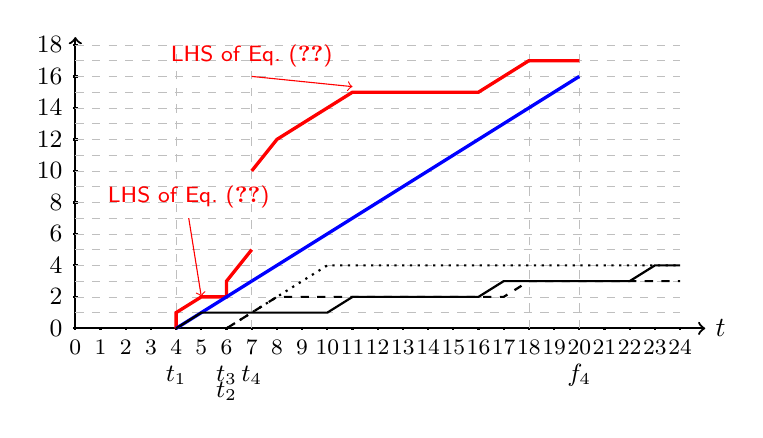
\begin{tikzpicture}[x=\ux,y=\uy, font=\sffamily,thick]  
		\tikzset{
			task/.style={fill=#1,  rectangle, text height=.3cm},
			task1a/.style={task=green!30},
			task1b/.style={task=green},
			task2a/.style={task=orange!30},
			task2b/.style={task=orange, minimum width=1mm},
			task3a/.style={task=pink, minimum width=1mm},
			task3b/.style={task=pink!80, minimum width=1mm},
			task4a/.style={task=cyan, minimum width=1mm},
			task4b/.style={task=cyan!50},
			task5/.style={task=blue},
			task6/.style={task=purple},
			task7/.style={minimum height=\ux,draw},
			task8/.style={minimum height=\ux,draw,thick},
			task9/.style={task=gray,minimum height=0.7cm,draw},
		}
		\tikzstyle{jobs}=[ fill=black!50];
		
		\draw[->] (0,0) -- coordinate (xaxis) (25,0) node[anchor=west] {$t$};
		\foreach \x in {0,...,24}{
			\draw[-](\x,0.1) -- (\x,-0.1)
			node[below] {\footnotesize $\x$};
			
		}
		\draw[->] (0,0) node[anchor=east] {}-- coordinate (xaxis) (0,18.5);
		\foreach \y in {0,2,...,18}{
			\draw[-](0.1, \y) -- (-0.1, \y)
			node[left] {\small $\y$};
			
		}

		\foreach \y in {1,2,...,18}{
                  \draw[-,very thin,lightgray, dashed](0,\y) -- (24,\y);
                }
		\foreach \x in {4,7,20,18}{
                  \draw[-,very thin,lightgray, dashed](\x,0) -- (\x,18);
                }
                  
                \draw (20, -3) node {\small $f_4$};
                \draw (7, -3) node {\small $t_4$};
                \draw (6, -3) node {\small $t_3$};
                \draw (6, -4) node {\small $t_2$};
                \draw (4, -3) node {\small $t_1$};

                \draw[->,red,thin](4.5, 7) node[anchor=south]{\footnotesize
                 LHS of Eq.~(\ref{eq:exec_plus_idle-2})} -- (5,2);
                \draw[-, very thick, red] (4,0) -- (4, 1) -- (5, 2) -- (6,2) -- (6, 3)
                -- (7, 5);
                \draw[->,red,thin](7, 16) node[anchor=south]{\footnotesize
                 LHS of Eq.~(\ref{eq:exec_plus_idle-3})} -- (11,15.35);
                \draw[-, very thick, red] (7, 10) -- (8, 12) -- (10, 14) -- (11,
                15) -- (16, 15) -- (17, 16) -- (18, 17) -- (20, 17);
                \draw[-, very thick, blue] (7,3) --(20,16);
                \draw[-, very thick, blue] (4,0) --(7,3);

                \draw[-,thick] (4,0) -- (5, 1) -- (10, 1) -- (11, 2) -- (16, 2)
                -- (17, 3) -- (22, 3) -- (23, 4) -- (24, 4);
                \draw[-,dashed] (6,0) -- (7, 1) -- (8, 2) -- (17, 2) -- (18, 3)
                -- (24, 3);
                \draw[-,dotted] (6,0) -- (10, 4) -- (24, 4);

		\end{tikzpicture}    
  \caption{\small The workload function for the three higher-priority tasks in Example~\ref{ex:proof_step1} when $\epsilon$ is very close to $0$. Solid black line: $W_1^1(t-t_1)$ when $t \geq t_1$, Dashed black line: $W_2^0(t-t_2)$ when $t \geq t_2$, Dotted black line: $W_3^1(t-t_3)$ when $t \geq t_3$, where the three workload functions are $0$ if $t-t_j < 0$ for $j=1,2,3$, Blue line (the only linear function from $t=4$ in this figure): $t-t_1$, Red line (marked by Eq.~\eqref{eq:exec_plus_idle-2} and Eq.~\eqref{eq:exec_plus_idle-3}): left-hand side of Eq.~(\ref{eq:exec_plus_idle-2}) when $t < 7$ and left-hand side of Eq.~(\ref{eq:exec_plus_idle-3}) when $ 7 \leq t < 20$.}
  \label{fig:example-step2}
\end{figure}



Lemma~\ref{lemma:conclusion-step2} may seem to provide a way to
construct the worst-case response time analysis of task
$\tau_k'$. However, it is not since $t_j$ values for $j=1,2,\ldots,k$
are in general unknown. We need to have a strategy to use the
conditions in Lemma~\ref{lemma:conclusion-step2} for analyzing a safe upper bound on the response time of $\tau_k'$.
Therefore, Step 3 has to construct a safe response-time analysis based on the
conditions specified by Eqs.~(\ref{eq:exec_plus_idle-2}) and
(\ref{eq:exec_plus_idle-3}) in Lemma~\ref{lemma:conclusion-step2}. Our
goal is to prove that the condition in
Eq.~\eqref{eq:TDA-suspension-tighter0} is more pessimistic than those
in Lemma~\ref{lemma:conclusion-step2} for any schedule $\Psi^1$ reduced from $\Psi$.

Towards this, we construct another release pattern
which moves $t_i$ to $t_i^*$ for $i=2,3,\ldots,k$ such that $t_i^*
\leq t_i$ and the corresponding conditions in Eqs.~(\ref{eq:exec_plus_idle-2}) and
(\ref{eq:exec_plus_idle-3}) will become worse when we use $t_i^*$. We start
the procedure as follows:
\begin{itemize}
\item Initial step: Let $t_1^*$ be $t_1$.
\item Iterative steps ($i=2,3,\ldots,k$): Let $t_i^*$ be $t_{i-1}^*+x_{i-1}\cdot\sigma_{i-1}$.
\end{itemize}
By the definition of $\sigma_i$, we know that $\sigma_i \leq t_{i+1}-t_i$ for $i=1,2,\ldots,k-1$.
Therefore,  for $i=2,3,\ldots,k$,\footnote{As already mentioned in Footnote~\ref{footnote-why-sigma}, if we used $S_j$ in Eqs.~(\ref{eq:exec_plus_idle-2}) and
(\ref{eq:exec_plus_idle-3}) instead of $\sigma_j$, this condition would not hold, and the proof would fall apart.}
\begin{equation*}
  t_i = t_1 + \sum_{j=1}^{i-1} (t_{j+1} - t_j) \geq t_1 + \sum_{j=1}^{i-1} x_j \sigma_j = t_i^*
\end{equation*}
since $x_j \in \{0, 1\}$ for any $j=1,2,\ldots,i-1$.

Figure~\ref{fig:example-proof-final} provides a concrete illustration about the procedure to define $t_1^*, t_2^*, t_3^*, t_4^*$ for the example used in Example~\ref{ex:proof_step1} when $\epsilon$ is close to $0$.
 Moreover, by
definition, $t_j^*$ is $t_1^* + \sum_{i=1}^{j-1} x_i\cdot\sigma_i$ for
$j=2,3,\ldots,k$.
For any task $\tau_j$ in ${\bf T}_1$,  $\forall \Delta \geq 0$, since $t_j \geq t_j^*$, we have
\begin{equation}
  \label{eq:execution-case1-shifted}
  W_j^1(\Delta)  \leq W_j^1(\Delta + (t_j-t_j^*)).
\end{equation}
For any task $\tau_j$ in ${\bf T}_0$,  $\forall \Delta \geq 0$, since $t_j \geq t_j^*$, we have
\begin{equation}
  \label{eq:execution-case2-shifted}
  W_j^0(\Delta)  \leq W_j^0(\Delta + (t_j-t_j^*)).
\end{equation}

\begin{figure}[t]
  \centering

		\def\ux{0.32cm}\def\uy{0.2cm} 
		\begin{tikzpicture}[x=\ux,y=\uy, font=\sffamily,thick]  
		\tikzset{
			task/.style={fill=#1,  rectangle, text height=.3cm},
			task1a/.style={task=green!30},
			task1b/.style={task=green},
			task2a/.style={task=orange!30},
			task2b/.style={task=orange, minimum width=1mm},
			task3a/.style={task=pink, minimum width=1mm},
			task3b/.style={task=pink!80, minimum width=1mm},
			task4a/.style={task=cyan, minimum width=1mm},
			task4b/.style={task=cyan!50},
			task5/.style={task=blue},
			task6/.style={task=purple},
			task7/.style={minimum height=\ux,draw},
			task8/.style={minimum height=\ux,draw,thick},
			task9/.style={task=gray,minimum height=0.7cm,draw},
		}
		\tikzstyle{jobs}=[ fill=black!50];
		
		\draw[->] (0,0) -- coordinate (xaxis) (25,0) node[anchor=west] {$t$};
		\foreach \x in {0,...,24}{
			\draw[-](\x,0.1) -- (\x,-0.1)
			node[below] {\footnotesize $\x$};
			
		}
		\draw[->] (0,0) node[anchor=east] {}-- coordinate (xaxis) (0,18.5);
		\foreach \y in {0,2,...,18}{
			\draw[-](0.1, \y) -- (-0.1, \y)
			node[left] {\small $\y$};
			
		}

		\foreach \y in {1,2,...,18}{
                  \draw[-,very thin,lightgray, dashed](0,\y) -- (24,\y);
                }
		\foreach \x in {4,7,20,18}{
                  \draw[-,very thin,lightgray, dashed](\x,0) -- (\x,18);
                }
                  
                \draw (20, -3) node {\small $f_4$};
                \draw (6, -3) node {\small $t_4^*$};
                \draw (5, -3) node {\small $t_3^*$};
                \draw (5, -4.5) node {\small $t_2^*$};
                \draw (4, -3) node {\small $t_1^*$};

                \draw[->,red,thin](5.5, 4) node[anchor=south,rotate=45,yshift=-0.1cm]{\footnotesize
                 LHS of Eq~\eqref{eq:exec_plus_idle-4}} -- (6.2,3.5);
                \draw[-,  very thick, red] (6, 3) -- (7,5);
                \draw[->,red,thin](8.4, 16.2) node[anchor=south]{\footnotesize
                 LHS of Eq.~(\ref{eq:exec_plus_idle-5}) and Eq.~\eqref{eq:exec_plus_idle-almost-final} when $t \geq 7$} -- (8,11.2);
                \draw[-, very thick, red] (7, 10) -- (9, 12) -- (10, 12) -- (11, 13) 
                -- (16, 13) -- (17, 15) -- (20, 15);
                \draw[-, very thick, blue] (6,0) --(20,14);
                \draw[-, very thick, cyan] (6,8) --(7,10);
                \draw[->,cyan](5.6, 10) node[anchor=south, rotate=45,xshift=-0.5cm, text width=2.5cm]{\footnotesize
                 LHS of Eq.~\eqref{eq:exec_plus_idle-almost-final} when $6 \leq t < 7$} -- (6.4,8.95);


               \draw[color=gray, dotted, very thick](6, 11) -- (7, 11) -- (7, 12) -- (10, 12) -- (10, 13) -- (16, 13) -- (16, 15) -- (20, 15);
               \draw[->,gray](17, 16.4) node[anchor=west,text width=2.5cm]{\footnotesize  LHS of Eq.~\eqref{eq:exec_plus_idle-almost-final-before-replacing-sigma} when $t=\theta+6$} -- (16,15.2);


                \draw[-,thick] (4,0) -- (5, 1) -- (10, 1) -- (11, 2) -- (16, 2)
                -- (17, 3) -- (22, 3) -- (23, 4) -- (24, 4);
                \draw[-,dashed] (5,0) -- (6, 1) -- (7, 2) -- (16, 2) -- (17, 3)
                -- (24, 3);
                \draw[-,dotted] (5,0) -- (9, 4) -- (23, 4) -- (24, 5);

		\end{tikzpicture}    
  \caption{\small The workload function for the three higher-priority tasks in Example~\ref{ex:proof_step1} when $\epsilon$ is very close to $0$. Solid black line: $W_1^1(t-t_1^*)$ when $t \geq t_1^*$, Dashed black line: $W_2^0(t-t_2^*)$ when $t \geq t_2^*$, Dotted black line: $W_3^1(t-t_3^*)$ when $t \geq t_3^*$, where the three workload functions are $0$ if $t-t_j^* < 0$ for $j=1,2,3$, Blue line (the only linear function from $t=6$ in this figure): $t-t_k^*=t-6$, Red line (marked by Eq.~\eqref{eq:exec_plus_idle-4} and Eq.~\eqref{eq:exec_plus_idle-5}): left-hand side of Eq.~(\ref{eq:exec_plus_idle-4}) when $t < 7$ and left-hand side of Eq.~(\ref{eq:exec_plus_idle-5}) and Eq.~\eqref{eq:exec_plus_idle-almost-final} when $ 7 \leq t < 20$, Purple line (marked by Eq.~\eqref{eq:exec_plus_idle-almost-final} when $6 \leq t < 7$), Gray dotted line (marked by Eq.~\eqref{eq:exec_plus_idle-almost-final-before-replacing-sigma}) by setting $\theta=t-6$.}
  \label{fig:example-proof-final}
\end{figure}


Therefore, for any $j=1,2,\ldots,k-1$, we know that $W_j^1(t-t_j)
\leq W_j^1(t-t_j^*)$ and $W_j^0(t-t_j) \leq W_j^0(t-t_j^*)$ for any $t
\geq t_j$. Putting Eqs.~\eqref{eq:execution-case1-shifted}~and~\eqref{eq:execution-case2-shifted} into 
Eq.~(\ref{eq:exec_plus_idle-2}) $\forall t \mid t_k^* \leq t < t_k$ leads to\footnote{This holds since the interval $[t_k^*, t_k]$ is fully covered by the interval $[t_1, t_k]$.}
{\small \begin{align}
&\sum_{j=1}^{k-1} x_j\cdot (W_j^1(t-t_j^*)+\sigma_j) + (1-x_j)\cdot W_j^0(t-t_j^*) \geq t-t_1,\nonumber\\
\Rightarrow& \sum_{j=1}^{k-1} x_j\cdot W_j^1(t-t_j^*) + (1-x_j)\cdot W_j^0(t-t_j^*) \geq t-t_k^*,
\label{eq:exec_plus_idle-4}
\end{align}}where $\Rightarrow$ is due to the condition
$t_k^* = t_1 + \sum_{j=1}^{k-1}x_j\sigma_j$.
Similarly, putting Eqs.~\eqref{eq:execution-case1-shifted}~and~\eqref{eq:execution-case2-shifted} into 
Eq.~(\ref{eq:exec_plus_idle-3}) $\forall t \mid t_k \leq t < f_k$ leads to 
\begin{equation}
\label{eq:exec_plus_idle-5}
C_k'+\sum_{j=1}^{k-1} x_j\cdot W_j^1(t-t_j^*) + (1-x_j)\cdot W_j^0(t-t_j^*) > t-t_k^*.
\end{equation}

The above two conditions in Eq.~\eqref{eq:exec_plus_idle-4} $\forall t \mid t_k^* \leq t < t_k$ and in Eq.~\eqref{eq:exec_plus_idle-5} $\forall t \mid t_k \leq t < f_k$ are very similar. If we put $C_k'$ to the left-hand side of Eq.~\eqref{eq:exec_plus_idle-4}, we can unify these two conditions into one due to the fact that $C_k' \geq C_k > 0$. Therefore, as an important intermediate step, we conclude the above discussions with the following lemma.

\begin{Lemma}
\label{lemma:step-3-one-condition}
Lemma~\ref{lemma:conclusion-step2} implies that
$\forall t \mid t_k^* \leq t < f_k$
\begin{equation}
\label{eq:exec_plus_idle-almost-final} 
C_k'+\sum_{j=1}^{k-1} x_j\cdot W_j^1(t-t_j^*) + (1-x_j)\cdot W_j^0(t-t_j^*) > t-t_k^*.
\end{equation}  
\end{Lemma}
\begin{proof}
  This is due to the above discussions for Eqs.~\eqref{eq:exec_plus_idle-4}~and~\eqref{eq:exec_plus_idle-5} and the fact $C_k' > 0$.
\end{proof}

\begin{Lemma}
\label{lemma:step-3-ceiling-condition}
Lemma~\ref{lemma:step-3-one-condition} implies that
$\forall \theta \mid 0 \leq \theta < f_k-t_k^*$
\begin{equation}
\label{eq:exec_plus_idle-almost-final-before-replacing-sigma} 
C_k'+\sum_{j=1}^{k-1} \ceiling{\frac{\theta+X_j+(1-x_j)(R_j-C_j)}{T_j}} C_j > \theta,
\end{equation}
where $X_j$ is $\sum_{\ell=j}^{k-1} x_\ell\sigma_\ell$. 
\end{Lemma}
\begin{proof}
  By the definition of $t_j^*$, $\forall t \mid t_k^* \leq t < f_k$,
  we have $t-t_j^* = t - t_k^* + \sum_{\ell=j}^{k-1}
  x_\ell\sigma_\ell = t-t_k^* + X_j$ for every $j=1,2,\ldots,k-1$. By using Lemma~\ref{lemma:W_0-and-W_1-upper} and $t-t_j^*$ above, we can rewrite the condition in Lemma~\ref{lemma:step-3-one-condition} as $\forall t \mid t_k^* \leq t < f_k$,
\begin{equation*}
C_k'+\sum_{j=1}^{k-1} \ceiling{\frac{t-t_k^*+X_j+(1-x_j)(R_j-C_j)}{T_j}} C_j > t-t_k^*
\end{equation*}

  By replacing $t-t_k^*$ with $\theta$, we reach the conclusion.
\end{proof}

% Therefore, for task $\tau_j$ in ${\bf T}_1$, we know that $\forall t
% \mid t_k^* \leq t < f_k$
% \begin{equation}\label{eq:upper-bound-Wj1}
% W_j^1(t-t_j^*) \leq \ceiling{\frac{t-t_j^*}{T_j}}C_j =
% \ceiling{\frac{t-t_k^* +\sum_{\ell=j}^{k-1} x_\ell\sigma_\ell}{T_j}}C_j  
% \end{equation}
%  Moreover, for task $\tau_j$ in ${\bf T}_0$ with $x_j = 0$,
% $\forall t
% \mid t_k^* \leq t < f_k$, we have 
% {\small \begin{align}
% W_j^0(t-t_j^*) & = W_j^0(t-t_k^* + t_k^* - t_j^*) = W_j^0(t-t_k^* + \sum_{\ell=j}^{k-1} x_\ell\sigma_\ell)\nonumber\\
% &\leq C_j + W_j^1(t-t_k^* + \sum_{\ell=j}^{k-1} x_\ell\sigma_\ell-(T_j-R_j+C_j))\nonumber\\
% & \leq \ceiling{\frac{t-t_k^*+\sum_{\ell=j}^{k-1} x_\ell\sigma_\ell +(R_j-C_j)}{T_j}}C_j  \label{eq:upper-bound-Wj0}
% \end{align}} Therefore, we can conclude that 
% $\forall t \mid t_k^* \leq t < f_k$
% \begin{equation}
% C_k'+\sum_{j=1}^{k-1} \ceiling{\frac{t-t_k^*+X_j+(1-x_j)(R_j-C_j)}{T_j}} C_j > t-t_k^*,
% \end{equation}
% where $X_j$ is $\sum_{\ell=j}^{k-1} x_\ell\sigma_\ell$. We replace $t-t_k^*$ with $\theta$. 

The condition in Lemma~\ref{lemma:step-3-ceiling-condition} implies that the minimum $\theta$ with $\theta > 0$ and
$C_k'+\sum_{j=1}^{k-1} \ceiling{\frac{\theta+X_j+(1-x_j)(R_j-C_j)}{T_j}} C_j = \theta$
 is larger than or equal to $f_k-t_k^* \geq f_k-t_k$. 
However, the condition in Lemma~\ref{lemma:step-3-ceiling-condition} requires the knowledge of $\sigma_i$. It is straightforward to see that $\sum_{j=1}^{k-1} \ceiling{\frac{\theta+X_j+(1-x_j)(R_j-C_j)}{T_j}} C_j$ reaches the worst case if $X_j$ is the largest. Since $X_j \leq Q_j^{\vec{x}}$ by using the last condition in Eq.~\eqref{eq:sumof-sigma} from Lemma~\ref{lem:max_idle}, we reach the conclusion of the correctness of Theorem~\ref{theorem:general-framework}, where  $Q_j^{\vec{x}}$ is defined in Theorem~\ref{theorem:general-framework}.

\hfill {\bf end of the proof of Theorem~\ref{theorem:general-framework}.} \qed  

\begin{example}
  We consider Example~\ref{ex:proof_step1} when $\epsilon$ is very
  close to $0$ to illustrate Step 3 in the proof of
  Theorem~\ref{theorem:general-framework}. For such a case, $t_1^*=4,
  t_2^*=5, t_3^*=5$, and $t_4^*=6$.
  Figure~\ref{fig:example-proof-final} presents the corresponding
  relations of the inequalities in Step 3. 
% be demonstrated in Figure~\ref{fig:example-proof-final} based on the
% previous example in
% Figure~\ref{fig:example}. Figure~\ref{fig:example-proof-final}
% provides the imaginary workload and an imaginary execution plan based
% on the test behind the condition in
% Eq.~\eqref{eq:exec_plus_idle-almost-final}. \emph{Note that this is
%   not an actual schedule since task $\tau_2$ is artificially alerted
%   to release two jobs within a short time interval. This is only for
%   illustrative purposes.}
% The two idle time units are used
% between time $4$ and time $6$. The accumulated workload is then
% started to be executed at time $6$ and the processor does not
% idle after time $6$. Over here, we see that two jobs of task $\tau_2$ are executed
% back to back from time 7 to time 9. As
% shown in the imaginary schedule in
% Figure~\ref{fig:example-proof-final}, the processor is busy executing
% the workload from time $6$ to time $21$, which is more pessimistic
% than the actual schedule in Figure~\ref{fig:example}. 
As shown in Figure~\ref{fig:example-proof-final}, all the inequalities 
  in Eqs.~\eqref{eq:exec_plus_idle-4},~\eqref{eq:exec_plus_idle-5},~\eqref{eq:exec_plus_idle-almost-final}, and~\eqref{eq:exec_plus_idle-almost-final-before-replacing-sigma} hold.
%The conclusion we have in the final statement of the example is that $20-7=f_k-r_k \leq  f_k-6 < 21-6$.
\end{example}
\vspace{-0.3in}
\end{appProof}


\begin{appProof}{of Theorem \ref{theorem:general-framework-not-feasible}}
  By the assumption that $R_k' > T_k$, there exists a schedule $\Psi$
  such that the response time of task $\tau_k$ is strictly larger than
  $T_k$. Let $J_k$ be the first job in the schedule $\Psi$ that has
  response time larger than $T_k$. Suppose that $J_{k}$ arrives at
  time $r_k$. When job $J_k$ is released at time $r_k$, there is no
  other unfinished jobs of task $\tau_k$. By
  Lemma~\ref{lemma:remove-same-task}, we can safely remove all the
  other jobs of task $\tau_k$ arrived before $r_k$ without affecting
  the response time of $J_k$. It is rather straightforward to see that
  removing all the other jobs of task $\tau_k$ arrived after $r_k$
  also does not change the fact that $J_k$ finishes after
  $r_k+T_k$. Let $f_k$ be the time at which $J_k$ finishes in the
  above schedule after removing the other jobs of task $\tau_k$. We
  know that $f_k - r_k > T_k$.

  Then, we can follow all the procedures and steps in the proof of
  Theorem~\ref{theorem:general-framework} to reach the same conclusion
  in Lemma~\ref{lemma:step-3-ceiling-condition}, which implies
  Theorem~\ref{theorem:general-framework-not-feasible} by setting $X_j
  \leq Q_j^{\vec{x}}$ for $j=1,2,\ldots,k-1$ since $f_k-r_k > T_k$ and
  $C_k'=C_k+S_k$.
\end{appProof}




%%% Local Variables:
%%% mode: latex
%%% TeX-master: "master.tex"
%%% End:
